\documentclass{article}
	
\usepackage{hyperref}
\usepackage{graphicx}
\usepackage{amsmath}
\usepackage[left=2cm, right=2cm, top=1cm, bottom = 1.5cm]{geometry}
\graphicspath{{Pictures/Plotting}}

\begin{document}
	
	In this document, we consider several classical systems and the phase lag they introduce.
	
	\section{Classical driven damped harmonic oscillator}
	
	Following \href{https://scholar.harvard.edu/files/schwartz/files/lecture2-driven-oscillators.pdf}{a lecture} from the internet, the equation of motion for the coordinate $ x = x (t) $ of the driven damped oscillator is
	
	\begin{equation}
	\ddot{x} + \gamma \dot{x} + \omega_0^2 x = \frac{1}{m} F(t). 
	\end{equation}
	
	We look for a steady-state solution of this equation, and find for $ z(t): x(t) = \Re[z(t)] $ when $F(t) = F_0\cos(\omega_d t)$:
	
	\begin{equation}
	z(t) = \frac{F_0}{m}\frac{1}{\omega_0^2 + i \gamma \omega_d - \omega_d^2} e^{i\omega_d t}
	\label{eq:zt}
	\end{equation}
	
	We have changed the sign of the anzatz function compared to the document; so as the time goes forward, the phase winds up. In \autoref{fig:driven-resonance}, we plot the amplitude and phase of $z(0)$ depending on the drive frequency.
	
	\begin{figure}[h!]
		\centering
		\includegraphics[width=\linewidth]{"Pictures/Plotting/driven resonance"}
		\caption{Amplitude and phase of the factor before the complex exponent in \autoref{eq:zt}  for $\omega_0/2\pi = $4 GHz, $\gamma = 100\  \text{us}^{-1}$, $ F_0/m = 1 $.}
		\label{fig:driven-resonance}
	\end{figure}

	Since $z(t) = |z(0)| e^{i(\omega_dt + \angle z(0) )}$, the solution for the real coordinate will be proportional to $\cos(\omega_d t + \angle z(0))$, and thus negative $\angle z(0)$ defines the lag of the oscillator before the driving force: in only reaches the same phase $F(t)$ just had in some positive time $|\angle z(0)|/\omega_d$.
	
	Therefore, signals emitted from the driven oscillator connected for example to a semi-infinite string should also be phase-delayed. However, we will discuss more involved cases in certain possible electrical schemes.
	
	\section{Fabri-Perot cavity}
	
	A similar situation we observe for a Fabri-Perot resonator. We define the electric field in a right propagating wave as 
	$E(x,t)^\rightarrow = \Re [E_0 e^{i(\omega t - k x)}].$ From here follows a standard expression for the transmission:
	
	\begin{equation}
		E_{out}(x,t) = E_0 \frac{t_1 t_2 e^{-ikl}}{1 - r_1 r_2 e^{-2 ikl}},
	\end{equation}
	
	where $t_{1,2}, r_{1,2} $ are the transparency and the reflectivity of the mirrors, $t_i^2+r_i^2 = 1$, and $ l $ is the cavity length. It may be obtained as follows. Immediately after the first mirror, we have transmitted field of $t_1 E_0$ without a phase shift. Upon passing through the cavity, it accumulates negative phase of $-ikl$. Right after the the second mirror, we find $E_0 t_1 t_2 e^{-ikl}$ -- this is the first term of the field going through. The other terms are obtained by taking into account the reflected waves inside the cavity. Reflection is described multiplying the field by a factor of $r_i e^{i \pi}$. Therefore, after a round trip and transmission through the second mirror again, we have $E_0 t_1 t_2 r_1 r_2 e^{-3ikl + 2i\pi}$. In overall, $E_{out}(x, t)$ is defined by the series :
	\begin{equation}
		E_{out}(x,t) = E_{in}(x,t) t_1 t_2 e^{-ikl} \sum_{m=0}^{\infty} r_1^m r_2^m  e^{-2m \cdot ikl}.
	\end{equation}
	
	Since to satisfy the wave equation in each of the 3 parts of the space separated by mirrors, $\omega = \frac{c}{n} k$ (linear dispersion in a medium with refractive index $n$), we can plot the transmission through the cavity depending on the ``driving frequency''. We do it in \autoref{fig:fabri-perot}. Note that from the definition of the right-propagating wave, the negative phase is equivalent to an additional spatial distance that wave has to travel. For the left-propagating wave the situation is the same but with negative spatial distance inserted. Negative phase addition always means that the wave is falling behind itself.
	
	\begin{figure}
		\centering
		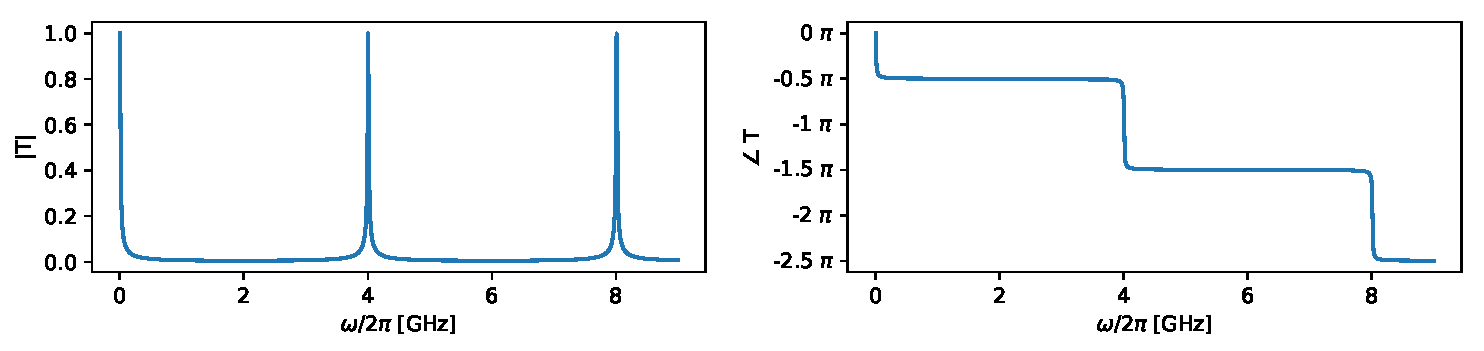
\includegraphics[width=1\linewidth]{Pictures/Plotting/fabri-perot}
		\caption{The transmission through the Fabri-Perot resonator. Note the similarity with \autoref{fig:driven-resonance}. However, at zero frequency in this case there is also a jump, which is not observed in a simple driven resonator. Also, an infinite number of modes is supported by the cavity. The parameters are $n = \sqrt{\frac{11.45+1}{2}}$, $l=15$ mm, $r_{1,2} = .99$ }
		\label{fig:fabri-perot}
	\end{figure}

	
	\section{Transmission line resonators}
	
	We first discuss the equivalent of the Fabri-Perot cavity, a piece of the transmission line of length $l$ coupled capacitively at the ends to two other semi-infinite transmission lines. The parameter $S_{21}$ is defined through the relation of the right-propagating waves in the left and in the right transmission lines.
	
	The circuit cimulator solves only for the real Kirchhoff voltages therefore it is necessary to use the following expression for the $S_{21} = 2 V_2 $, where $V_2$ is the voltage at the output resistor. It is easy to check that for a short instead of the transmission line in the left panel of \autoref{fig:tl1} one obtains $ S_{21}  = 1$.
	
	\begin{figure}[h!]
		\centering
		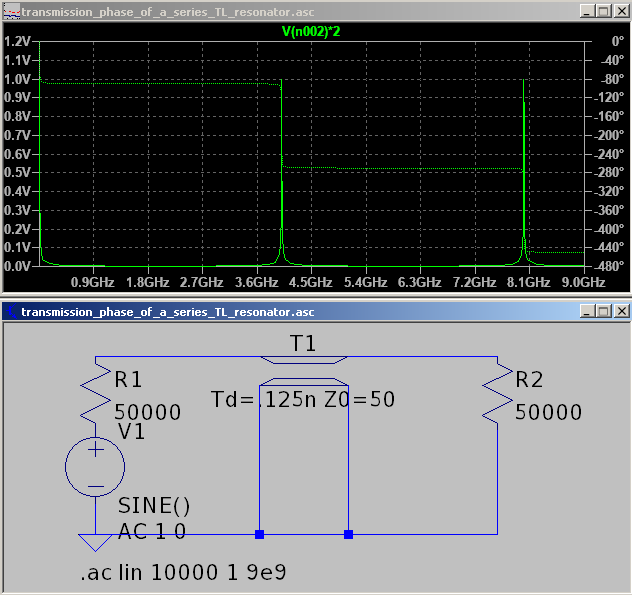
\includegraphics[width=0.45\linewidth]{Pictures/Plotting/TL1}
		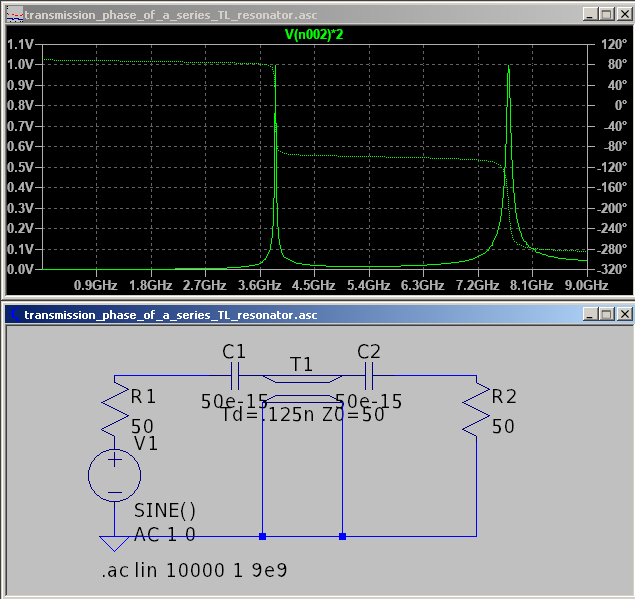
\includegraphics[width=0.45\linewidth]{Pictures/Plotting/TL2}
		\caption{\textbf{Left.}  Simulation of an idealized electrical circuit showing the transmission line with unmatched impedances, causing reflections at its ends described by $r_{1,2} = \frac{Z_0 - Z_{1,2}}{Z_0 + Z_{1,2}}$. Transmission coefficient is fully equivalent to the Fabri-Perot case. \textbf{Right.} The real setup where two 50-ohm transmission lines are coupled to the resonator via capacitive couplers. Note that now the linewidths depends on the mode number, and there is no transmission at zero frequency.}
		\label{fig:tl1}
	\end{figure}
	
	As one can see from \autoref{fig:tl1}, the phase of the S-parameter always goes down when passing through the resonance, which is obviously corresponding to the previous cases.
	
	
\end{document}